\section{Storage systems}

Storage systems can be classified into three main categories:
\begin{itemize}
    \item \textit{Direct Attached Storage} (DAS): these storage systems are directly linked to a server or workstation, appearing as disks within the client operating system.
    \item \textit{Network Attached Storage} (NAS):a computer connected to a network, offering file-based data storage services to other devices on the network.
    \item \textit{Storage Area Networks} (SAN): remote storage units connected to servers through specific networking technologies.
\end{itemize}
\begin{figure}[H]
    \centering
    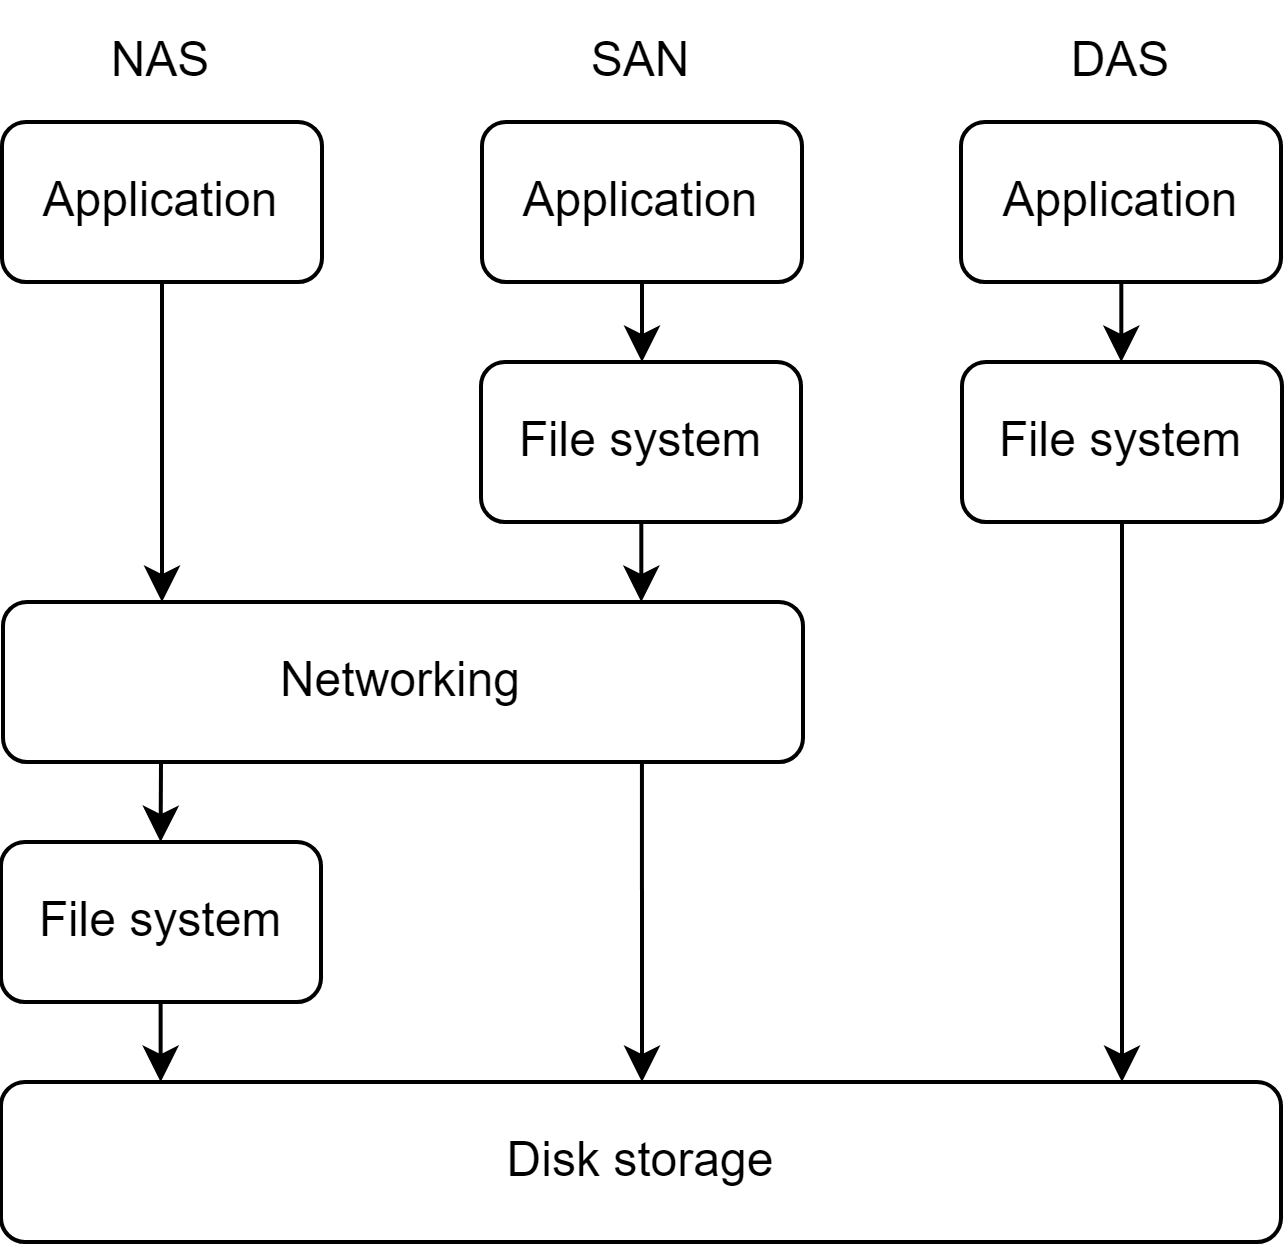
\includegraphics[width=0.6\linewidth]{images/ssc.png}
    \caption{Storage system classification}
\end{figure}

\subsection{Direct Attached Storage}
Direct Attached Storage (DAS) refers to storage systems directly connected to a server or workstation. 
Key characteristics of DAS include limited scalability and complex manageability. 
Accessing files from other machines typically requires utilizing the file-sharing protocol of the operating system. 
DAS can be internal or external; any external disks connected via a point-to-point protocol to a PC can be classified as DAS.
\begin{figure}[H]
    \centering
    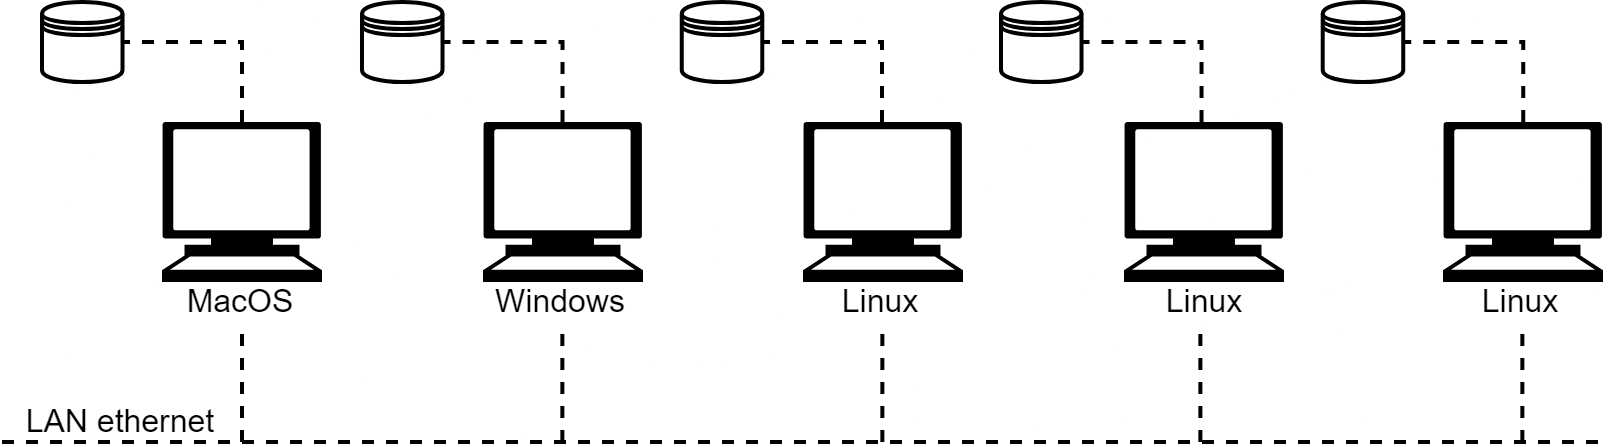
\includegraphics[width=0.75\linewidth]{images/das.png}
    \caption{DAS architecture}
\end{figure}

\subsection{Network Attached Storage}
A Network Attached Storage (NAS) unit is a computer connected to a network, offering file-based data storage services exclusively to other devices within the network. 
NAS systems typically comprise one or more hard disks, often configured into logical redundant storage containers or RAID setups. 
They provide file-access services to hosts connected via TCP/IP networks through protocols like Networked File Systems or SAMBA. 
Each NAS element is assigned its own IP address, facilitating individual identification and management. 
NAS systems exhibit good scalability, allowing for the addition of devices within each NAS element or the expansion of the number of NAS elements themselves.
\begin{figure}[H]
    \centering
    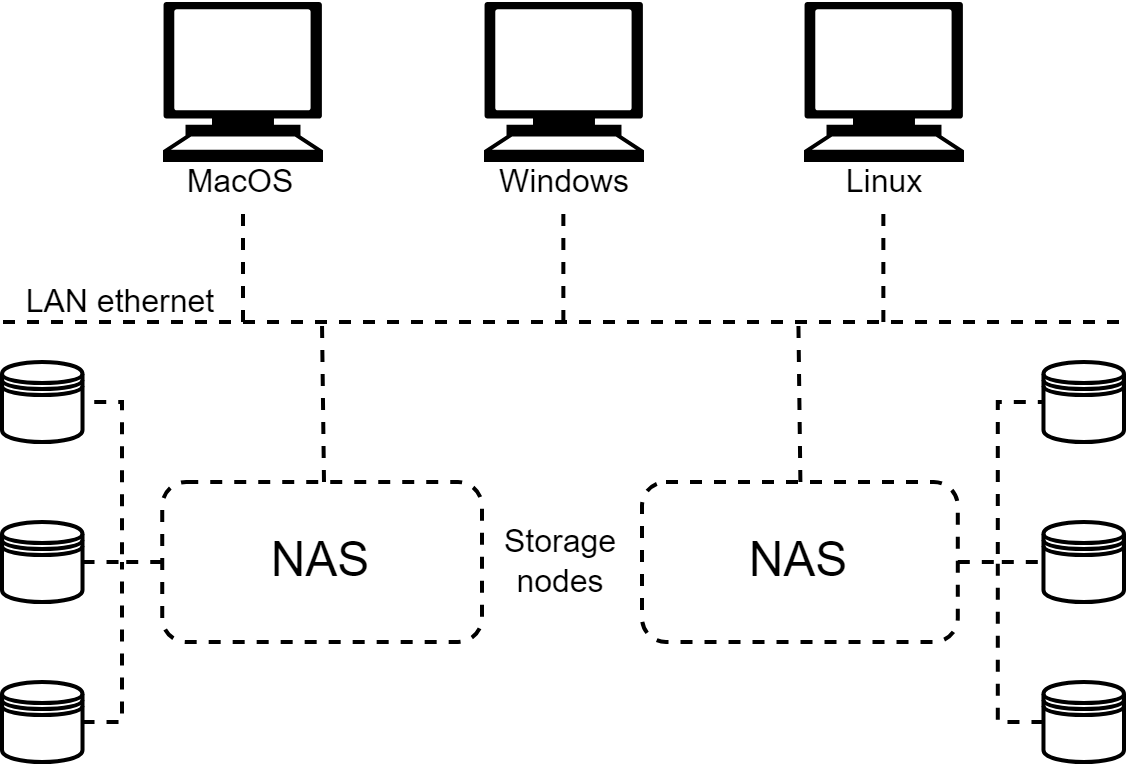
\includegraphics[width=0.6\linewidth]{images/nas.png}
    \caption{NAS architecture}
\end{figure}

\subsection{Storage Area Network}
Storage Area Networks (SANs) are remote storage units connected to PCs/servers through specific networking technologies. 
SANs feature a dedicated network solely devoted to accessing storage devices, typically comprising two distinct networks: one for TCP/IP communication and another dedicated network, like fiber channel. 
They offer high scalability by simply increasing the number of storage devices connected to the SAN network.
\begin{figure}[H]
    \centering
    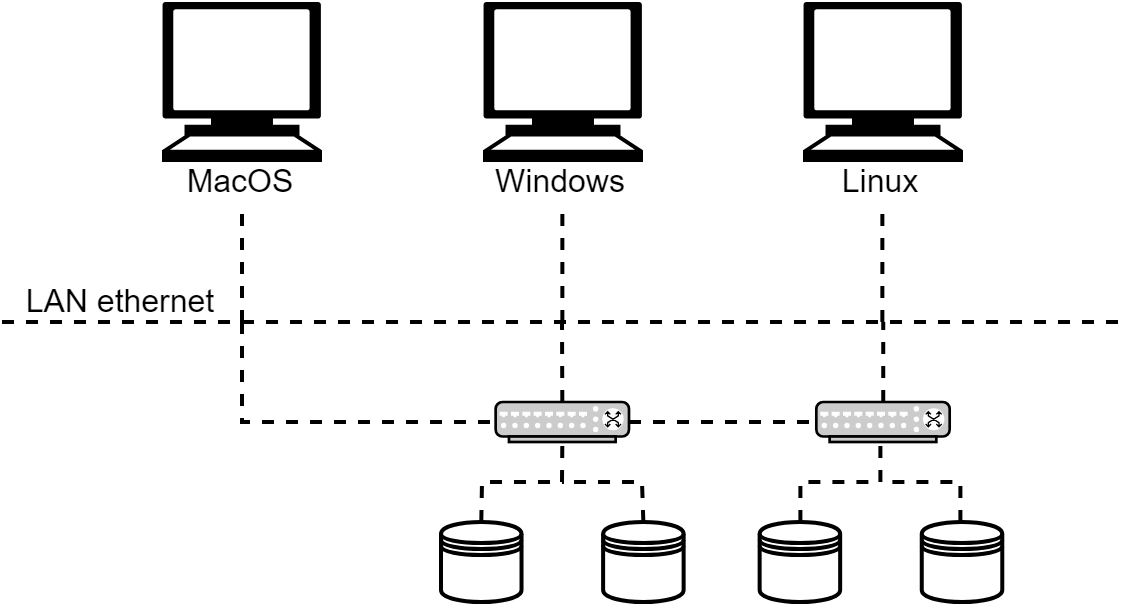
\includegraphics[width=0.6\linewidth]{images/san.png}
    \caption{Storage Area Network architecture}
\end{figure}

\subsection{Summary}
\paragraph*{NAS and DAS}
The primary distinctions between NAS and DAS lie in their design and functionality. 
DAS operates as an extension of an existing server and is not necessarily networked. 
It is directly connected to a server or workstation, appearing as local disks or volumes within the client operating system. 
In contrast, NAS is intentionally designed as a convenient, self-contained solution for sharing files across a network. It connects to the network, offering file-based data storage services to multiple devices. 
The performance of NAS is primarily dependent on the network's speed and congestion levels.

\paragraph*{NAS and SAN}
NAS and SAN differ fundamentally in their storage and file system provisions. 
NAS offers both storage and a file system, presenting itself to the client OS as a file server. 
This allows clients to map network drives to shares on the NAS server. On the other hand, SAN provides only block-based storage, leaving file system management to the client side. 
A disk accessed through SAN appears to the client OS as a local disk, visible in disk and volume management utilities and available for formatting with a file system.

Traditionally, NAS is used for low-volume access to a large amount of storage by many users, making it suitable for file storage and sharing in big data applications. 
In contrast, SAN is designed for high-performance environments, such as database management systems (DBMS) and virtual environments, where petabytes of storage and simultaneous access to files are required, such as in streaming audio and video.
\begin{table}[H]
    \centering
    \begin{tabular}{|c|lll|}
    \hline
                       & \multicolumn{1}{c}{\textbf{Application domain}}                                                        & \multicolumn{1}{c}{\textbf{Advantages}}                                                                                                                  & \multicolumn{1}{c|}{\textbf{Disadvantages}}    \\ \hline
    \textit{DAS}       & \makecell{Budget constraints \\ Simple storage solutions} & \makecell{Easy setup \\ Low cost \\ High performance}                           & \makecell{Limited accessibility \\ Limited scalability \\ No central management} \\\hline
    \textit{NAS}       & \makecell{File storage and sharing \\ Big data}           & \makecell{Scalability \\ Greater accessibility \\ Performance}                  & \makecell{Increased LAN traffic \\ Performance limitations \\ Security and reliability}     \\ \hline
    \textit{SAN}       & \makecell{DBMS \\ Virtual environments}                   & \makecell{Improved performance \\ Greater scalability \\ Improved availability} & \makecell{Costs \\ Complex setup and maintenance}           \\ \hline                                                            
    \end{tabular}
\end{table}